\subsection{Estimation of fANOVA decomposition}
The fANOVA decomposition has a strong theoretical foundation but especially in modern work, estimation approaches and computational feasibility is an important aspect to consider.
Also we saw that obtaining the fANOVA components analytically is not always possible, especially under dependent inputs. Therefore, we need to look at estimation approaches that allow us to compute the fANOVA components from data.

\subsubsection*{Estimation based on Partial Dependence}
In his estimation framework \cite{hooker2004} picks up the role of projections in fANOVA. To obtain the component estimate for $y_u$, he proposes to estimate the projections of $y$ onto the subspace of variables spanned by $u$ empirically.
More concretely, one first estimates the conditional expected value of the variables in $u$ (keep variables in $u$ fixed an average over all others). This is a simple Monte Carlo estimation, which results in the partial dependence function (PD Function) for the variables in $u$ \citep{hooker2004}.
The PD Function can then be used to estimate the empirical projection of interest. He states that his method works well for functions that have a nearly additive true structure and purely additive functions are exactly recoverable with this approach. To save computational costs, he proposes to base the Monte Carlo estimates of the PD function on a randomly sampled subset of data points.
Problem: no true projections (under dependence or always?); extrapolation issues etc.; even if no product type measure assumption, still problems in handling dependent inputs.

\subsubsection*{Estimation based on weighted least squares}
\cite{hooker2007} proposes a new estimation scheme for his generalized fANOVA decomposition. The mathematical problem one faces is more complex: the fANOVA components are defined in dependence of each other and system has to be solved simultaneously as we saw in the previous section.
Hooker rewrites the estimation problem as a restricted weighted least squares problem and solves it via Lagrange multiplier for the exact solution of the simultaneously defined generalized components; problem restricted to ensure hierarchical orthogonality.
The function is again evaluated at a grid of points to reduce the problem to a finite dimensional one. 
Because of the parallel to weighted least squares, it is also possible to compute a weighted standard ANOVA with existing software, but it is difficult to incorporate the constraints, so the components may not be hierarchical orthogonal.

\subsubsection*{Estimation based on polynomial expansion}
\cite{rahman2014} approaches the estimation differently and represents each component with a Fourier polynomial expansion. For normally distributed inputs, one can choose Hermit polynomials as basis functions, which simplifies things; in other cases more complicated I think.
Again need to look up the mechanisms better.
Other work, quiet mathematical that also goes in this direction I think.

No standard implementations available. Use existing software for parts (e.g. Monte Carlo estimates) and workarounds.

\subsection{Examples of fANOVA decomposition}
% Known function, simulate input, plot fANOVA and PD, comparison

% PD and fANOVA: If inputs are independent, I think for the main effects fANOVA is simply PD shifted but fANOVA answers a different question than PD. PD usually asks for the effect of one specific variable on the prediction. In contrast, fANOVA decomposes the entire function. It is more about a global representation and clean, isolated effects because in sum they have to recover the original function and may not overlap.

\subsubsection*{Standard MVN, linear function, interaction}
Let us recall the fANOVA components from our first example of function $g(x_1, x_2) = x_1 + 2 x_2 + x_1 x_2$ under independence:
\begin{align*}
y_{\emptyset} &= 0, \\
y_1(x_1) &= x_1\\
y_2(x_2) &= 2x_2\\
y_{12}(x_1, x_2) &= x_1x_2.
\end{align*}
We can plot the main effects and the contour plot of the interaction term:
% Input: MVN, centred, independent
\begin{figure}[htpb]
    \centering
    \begin{minipage}[t]{0.49\textwidth}
        \centering
        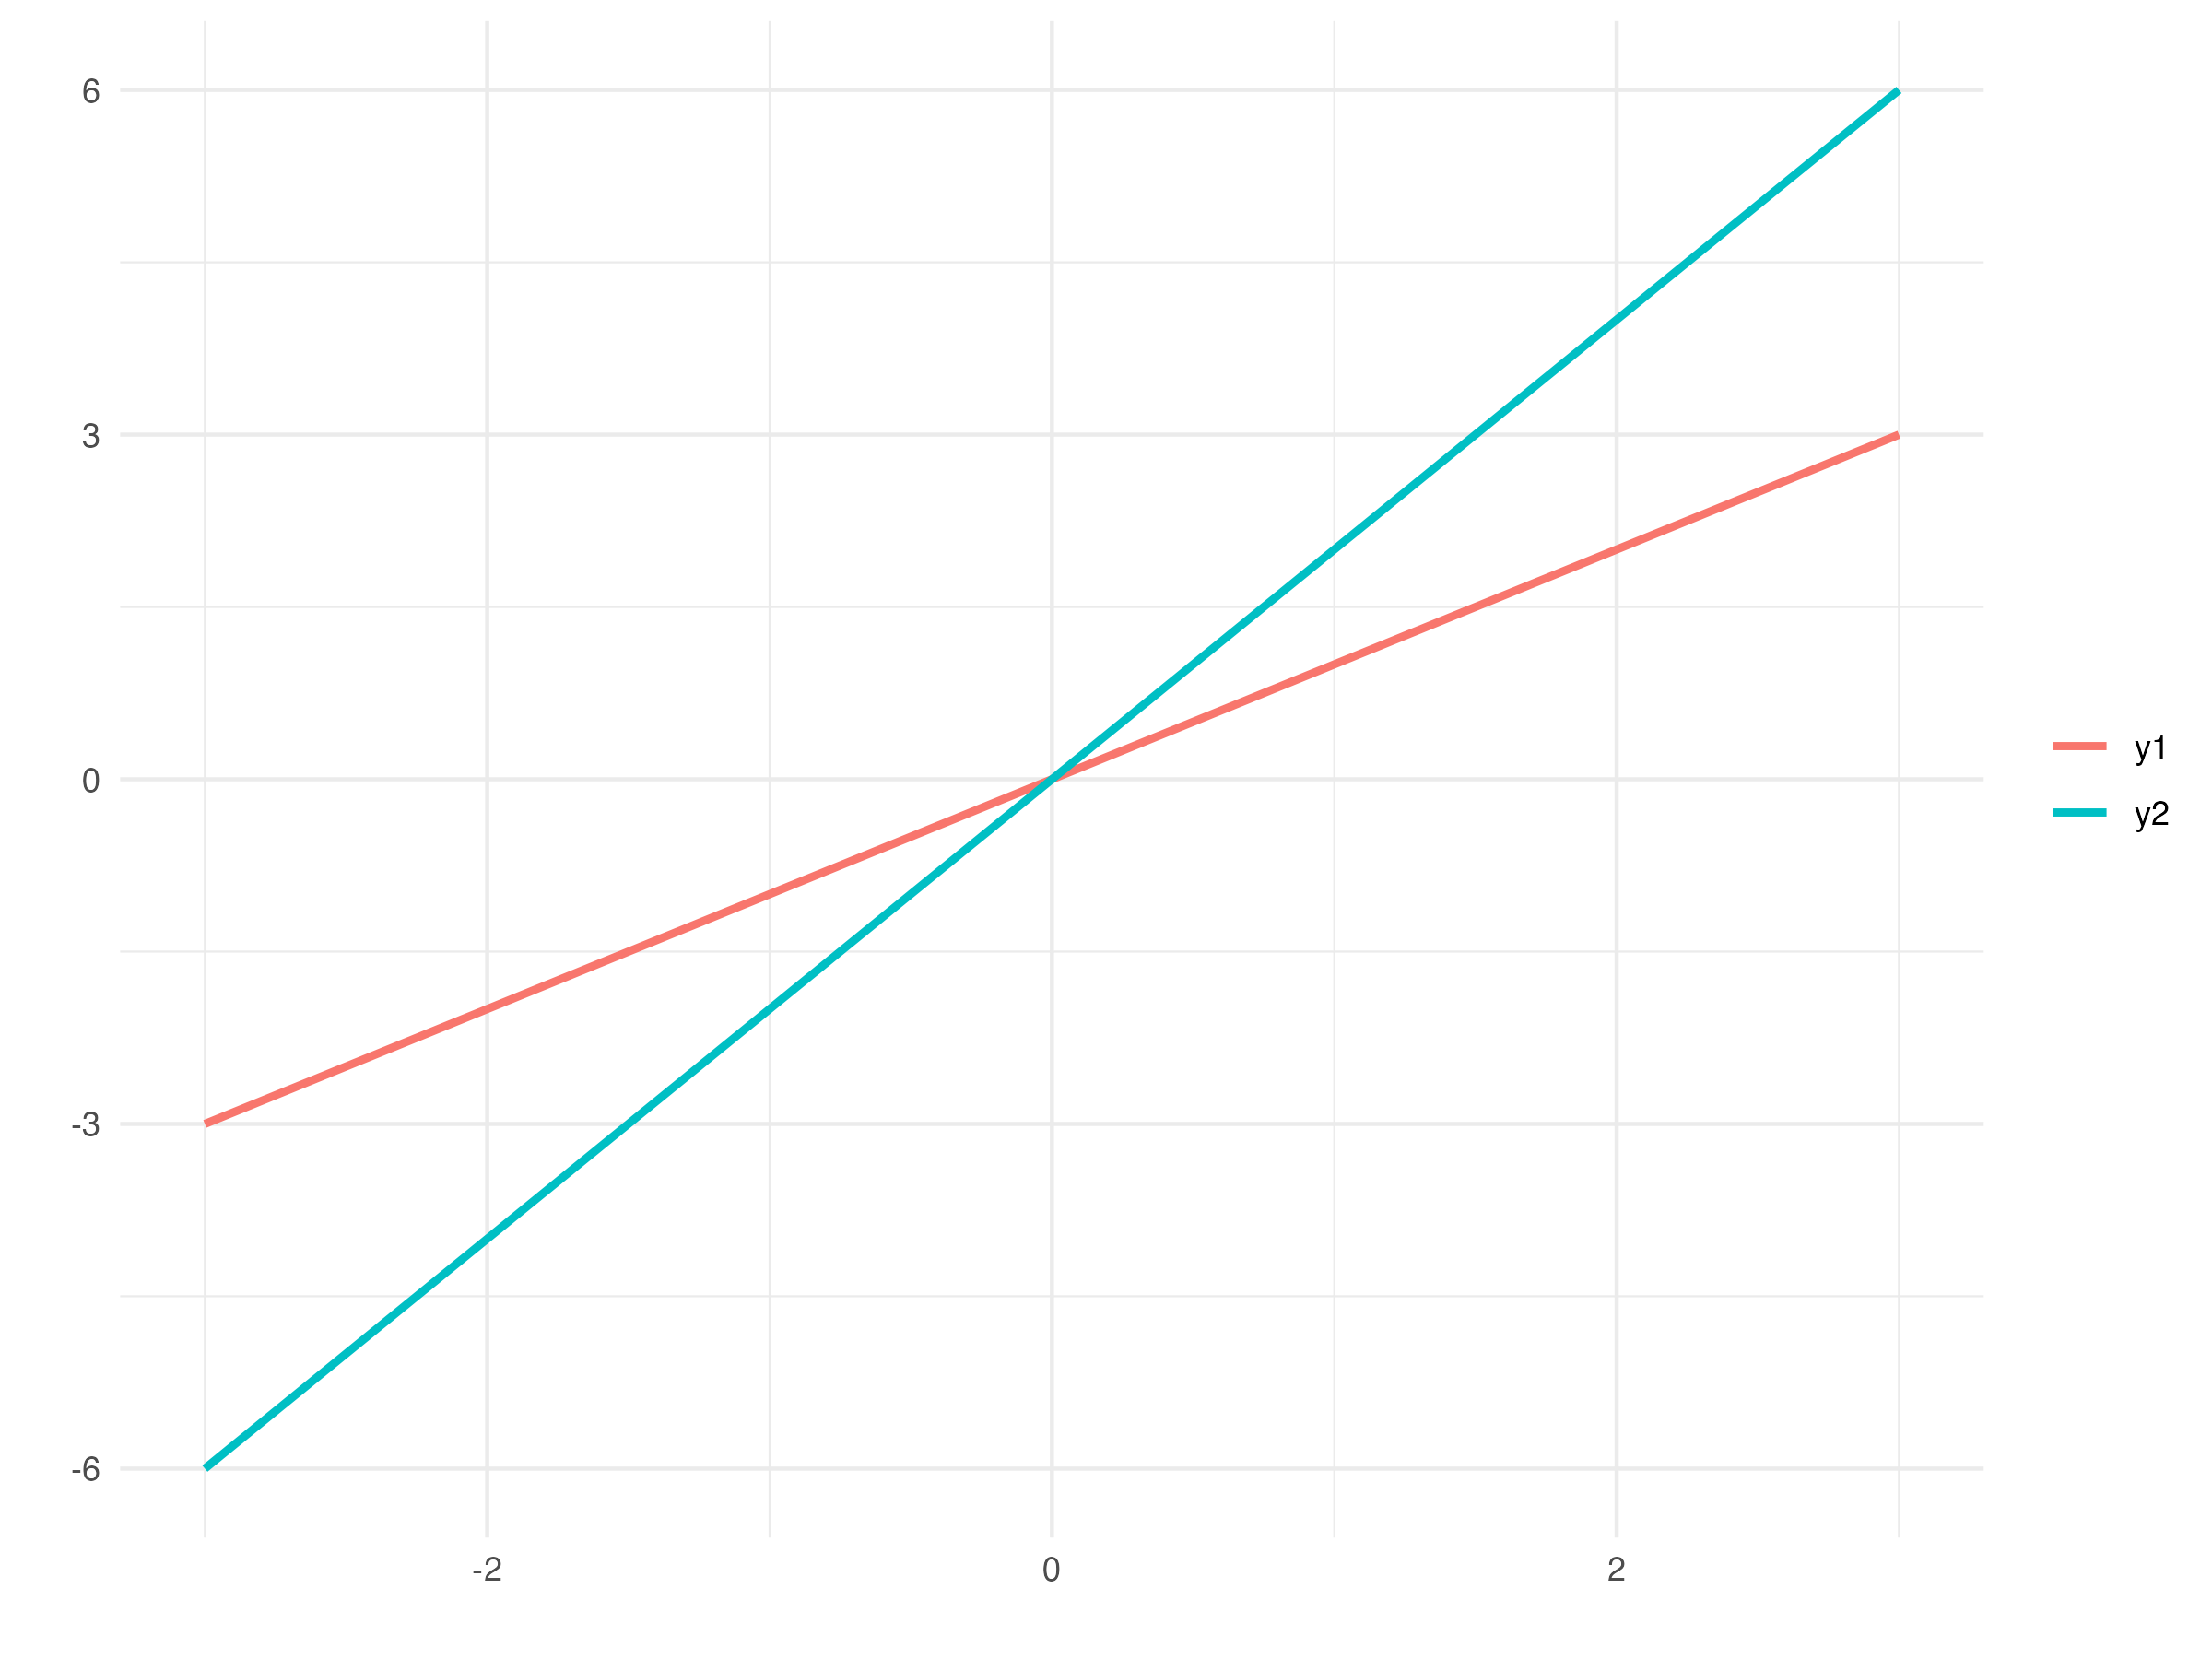
\includegraphics[width=\textwidth]{images/p_main_effect_ex1.png}
        \caption{Main terms as calculated via classical fANOVA for $g(x) = x_1 + 2 x_2 + x_1 x_2$.}
        \label{fig:main_effects_ex1}
    \end{minipage}%
    \hfill
    \begin{minipage}[t]{0.49\textwidth}
        \centering
        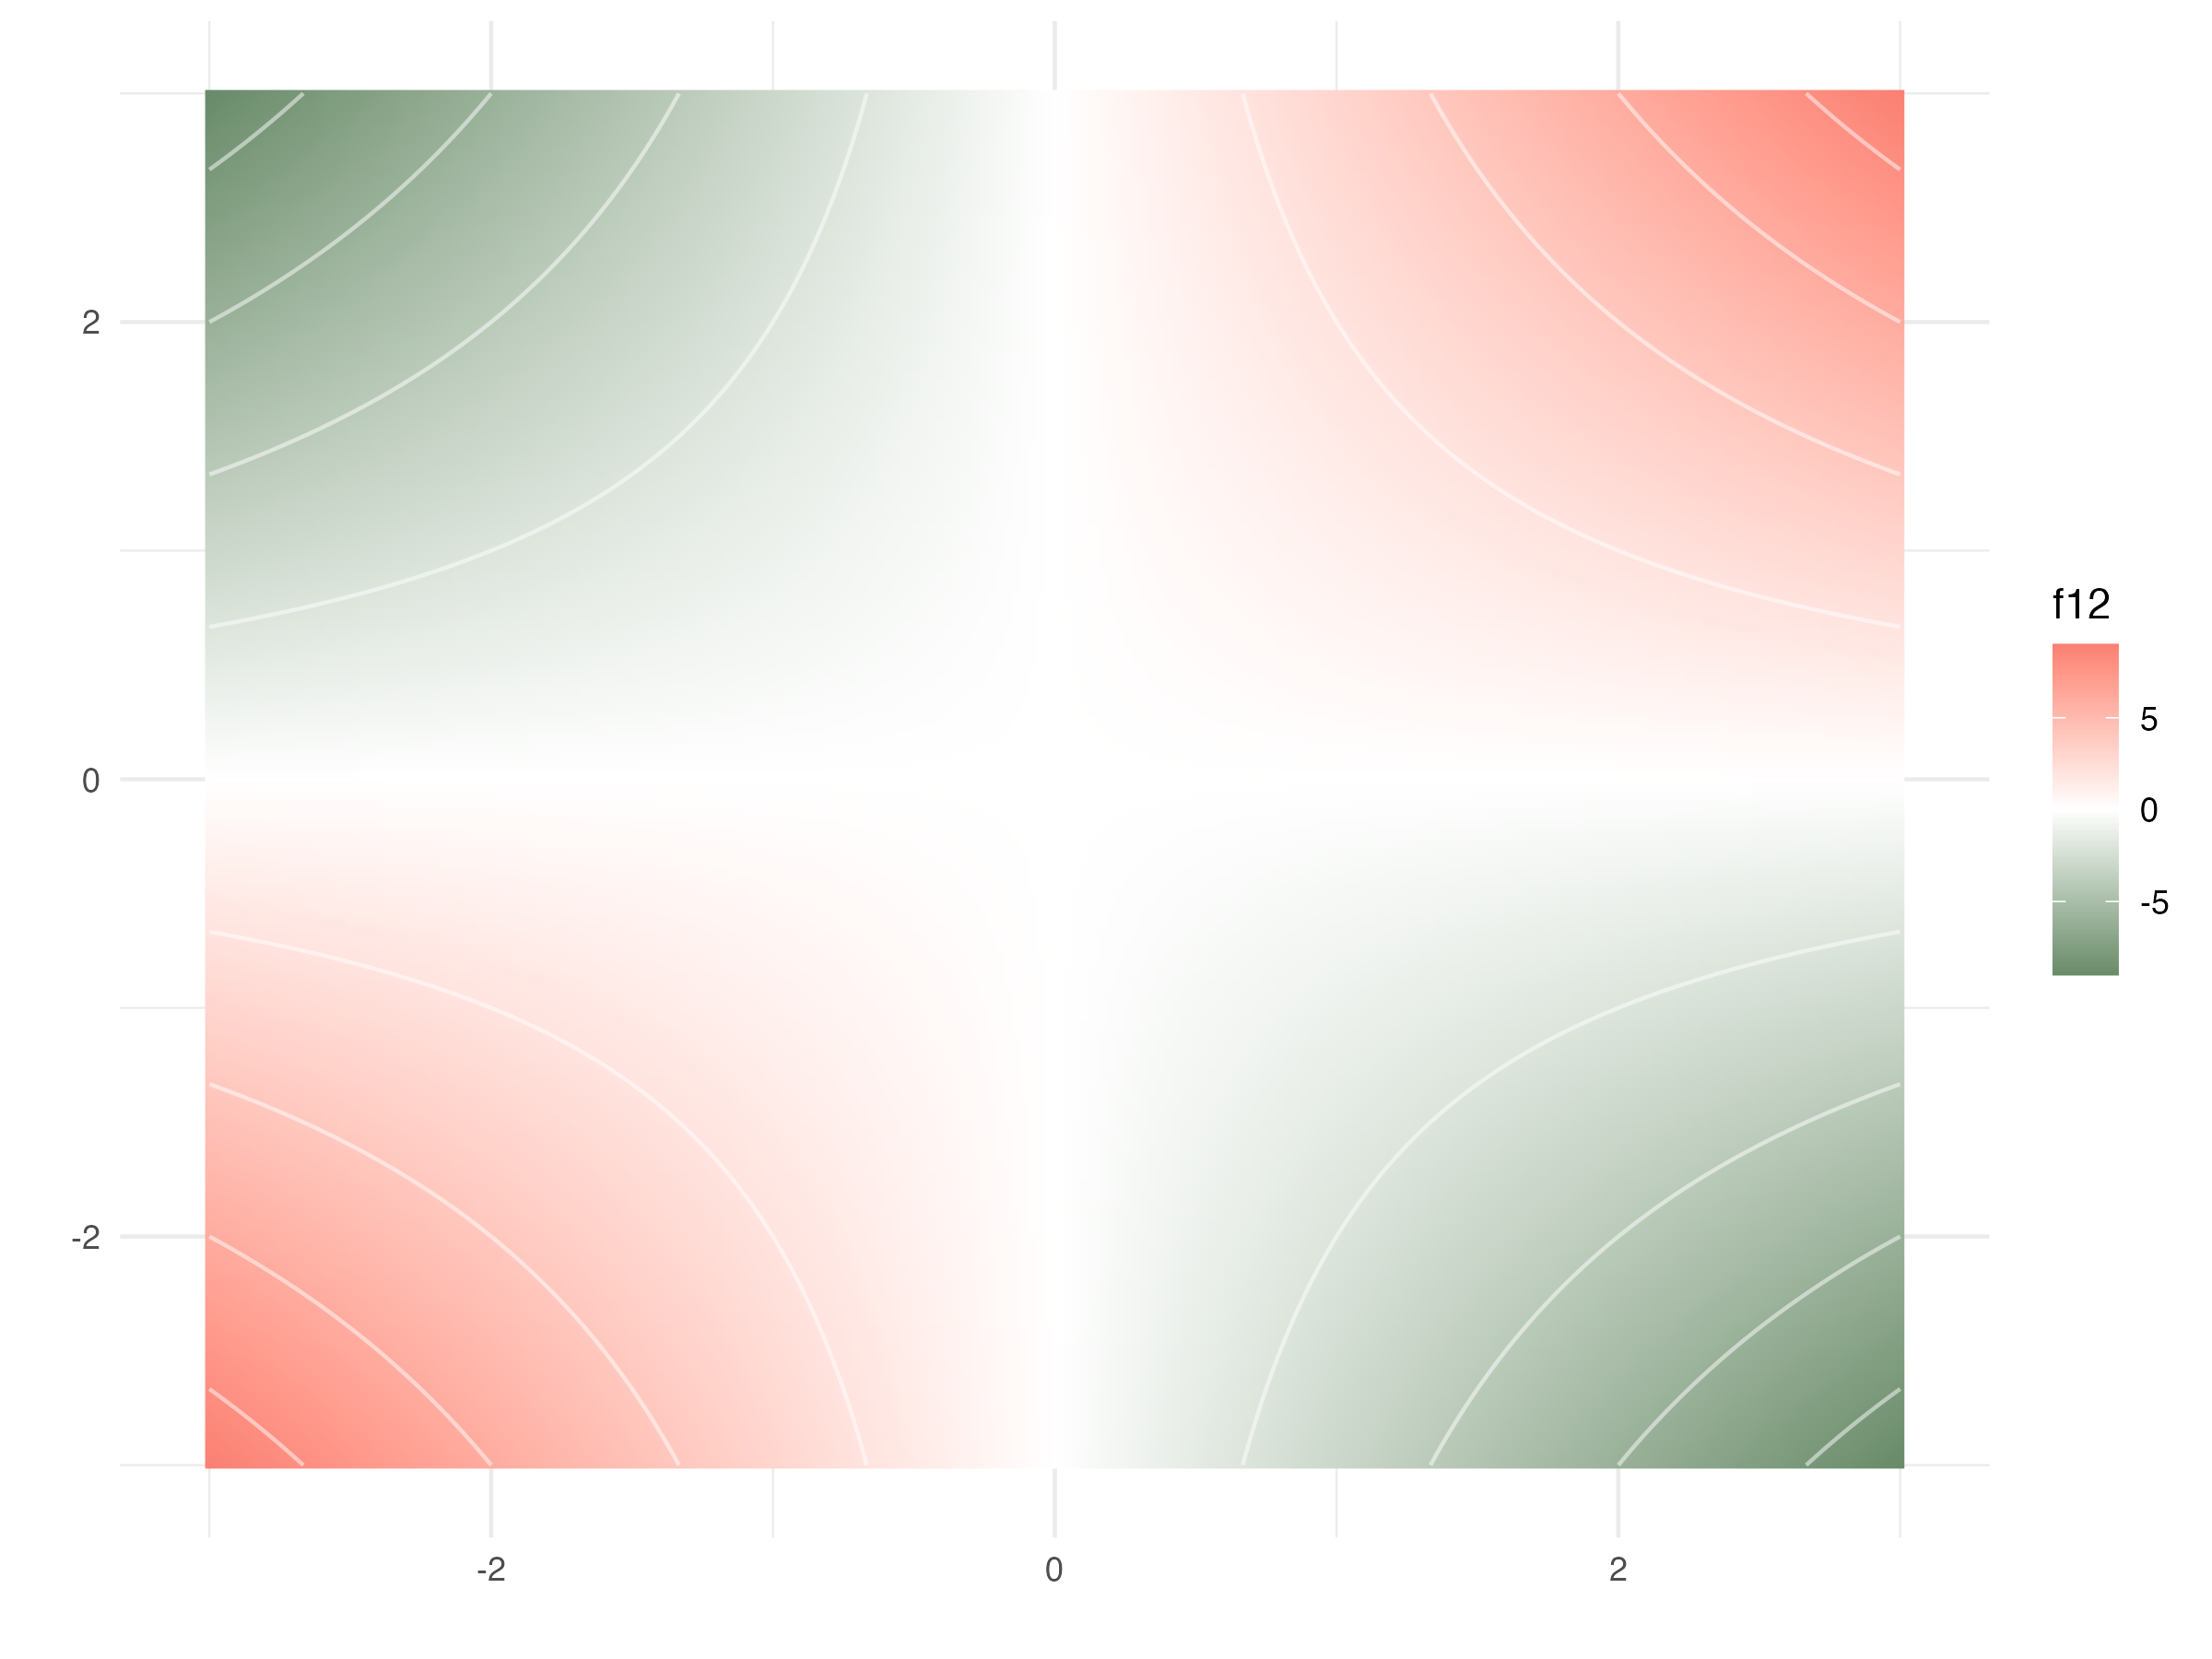
\includegraphics[width=\textwidth]{images/p_contour_ex1.png}
        \caption{Contour plot of $g(x) = x_1 + 2 x_2 + x_1 x_2$.}
        \label{fig:contour_ex1}
    \end{minipage}
\end{figure}

% \begin{figure}[htpb]
%     \centering
%     \begin{minipage}[t]{0.49\textwidth}
%         \centering
%         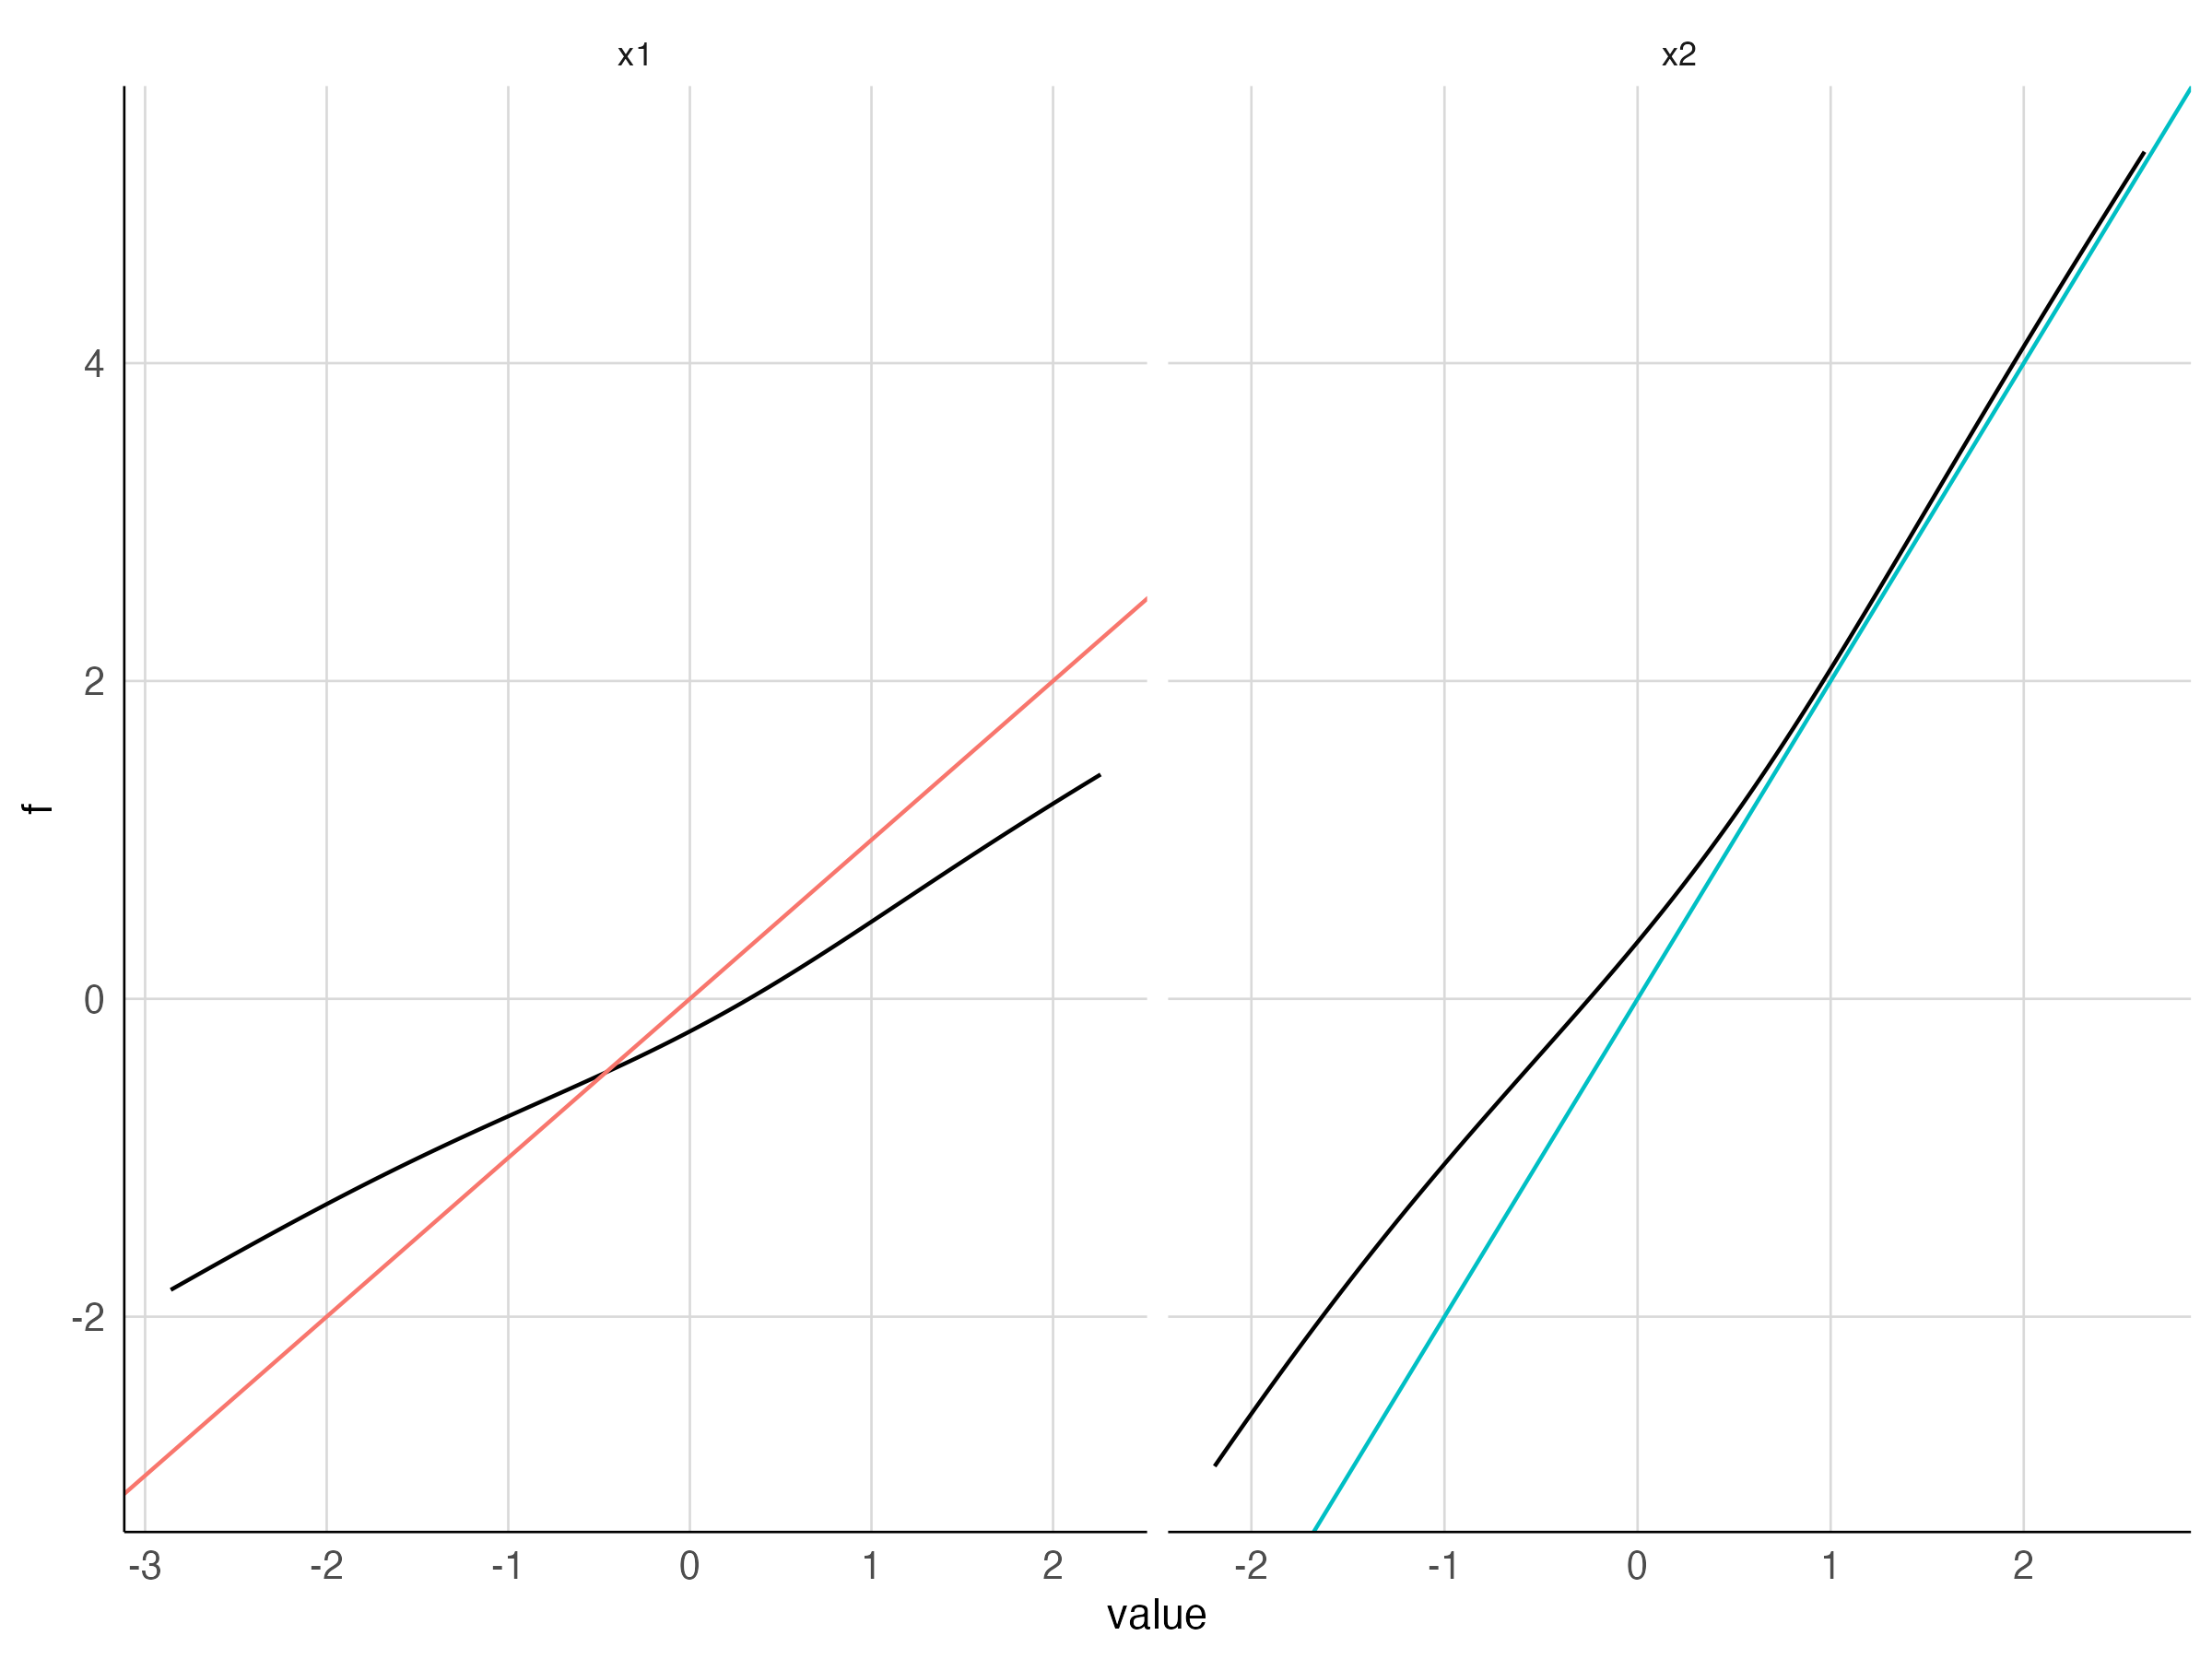
\includegraphics[width=\textwidth]{images/indep_150_main.png}
%         \caption{Estimation of Main terms as calculated via classical fANOVA for $g(x) = x_1 + 2 x_2 + x_1 x_2$ via Hooker method.}
%         \label{fig:indep_150_main}
%     \end{minipage}%
%     \hfill
%     \begin{minipage}[t]{0.49\textwidth}
%         \centering
%         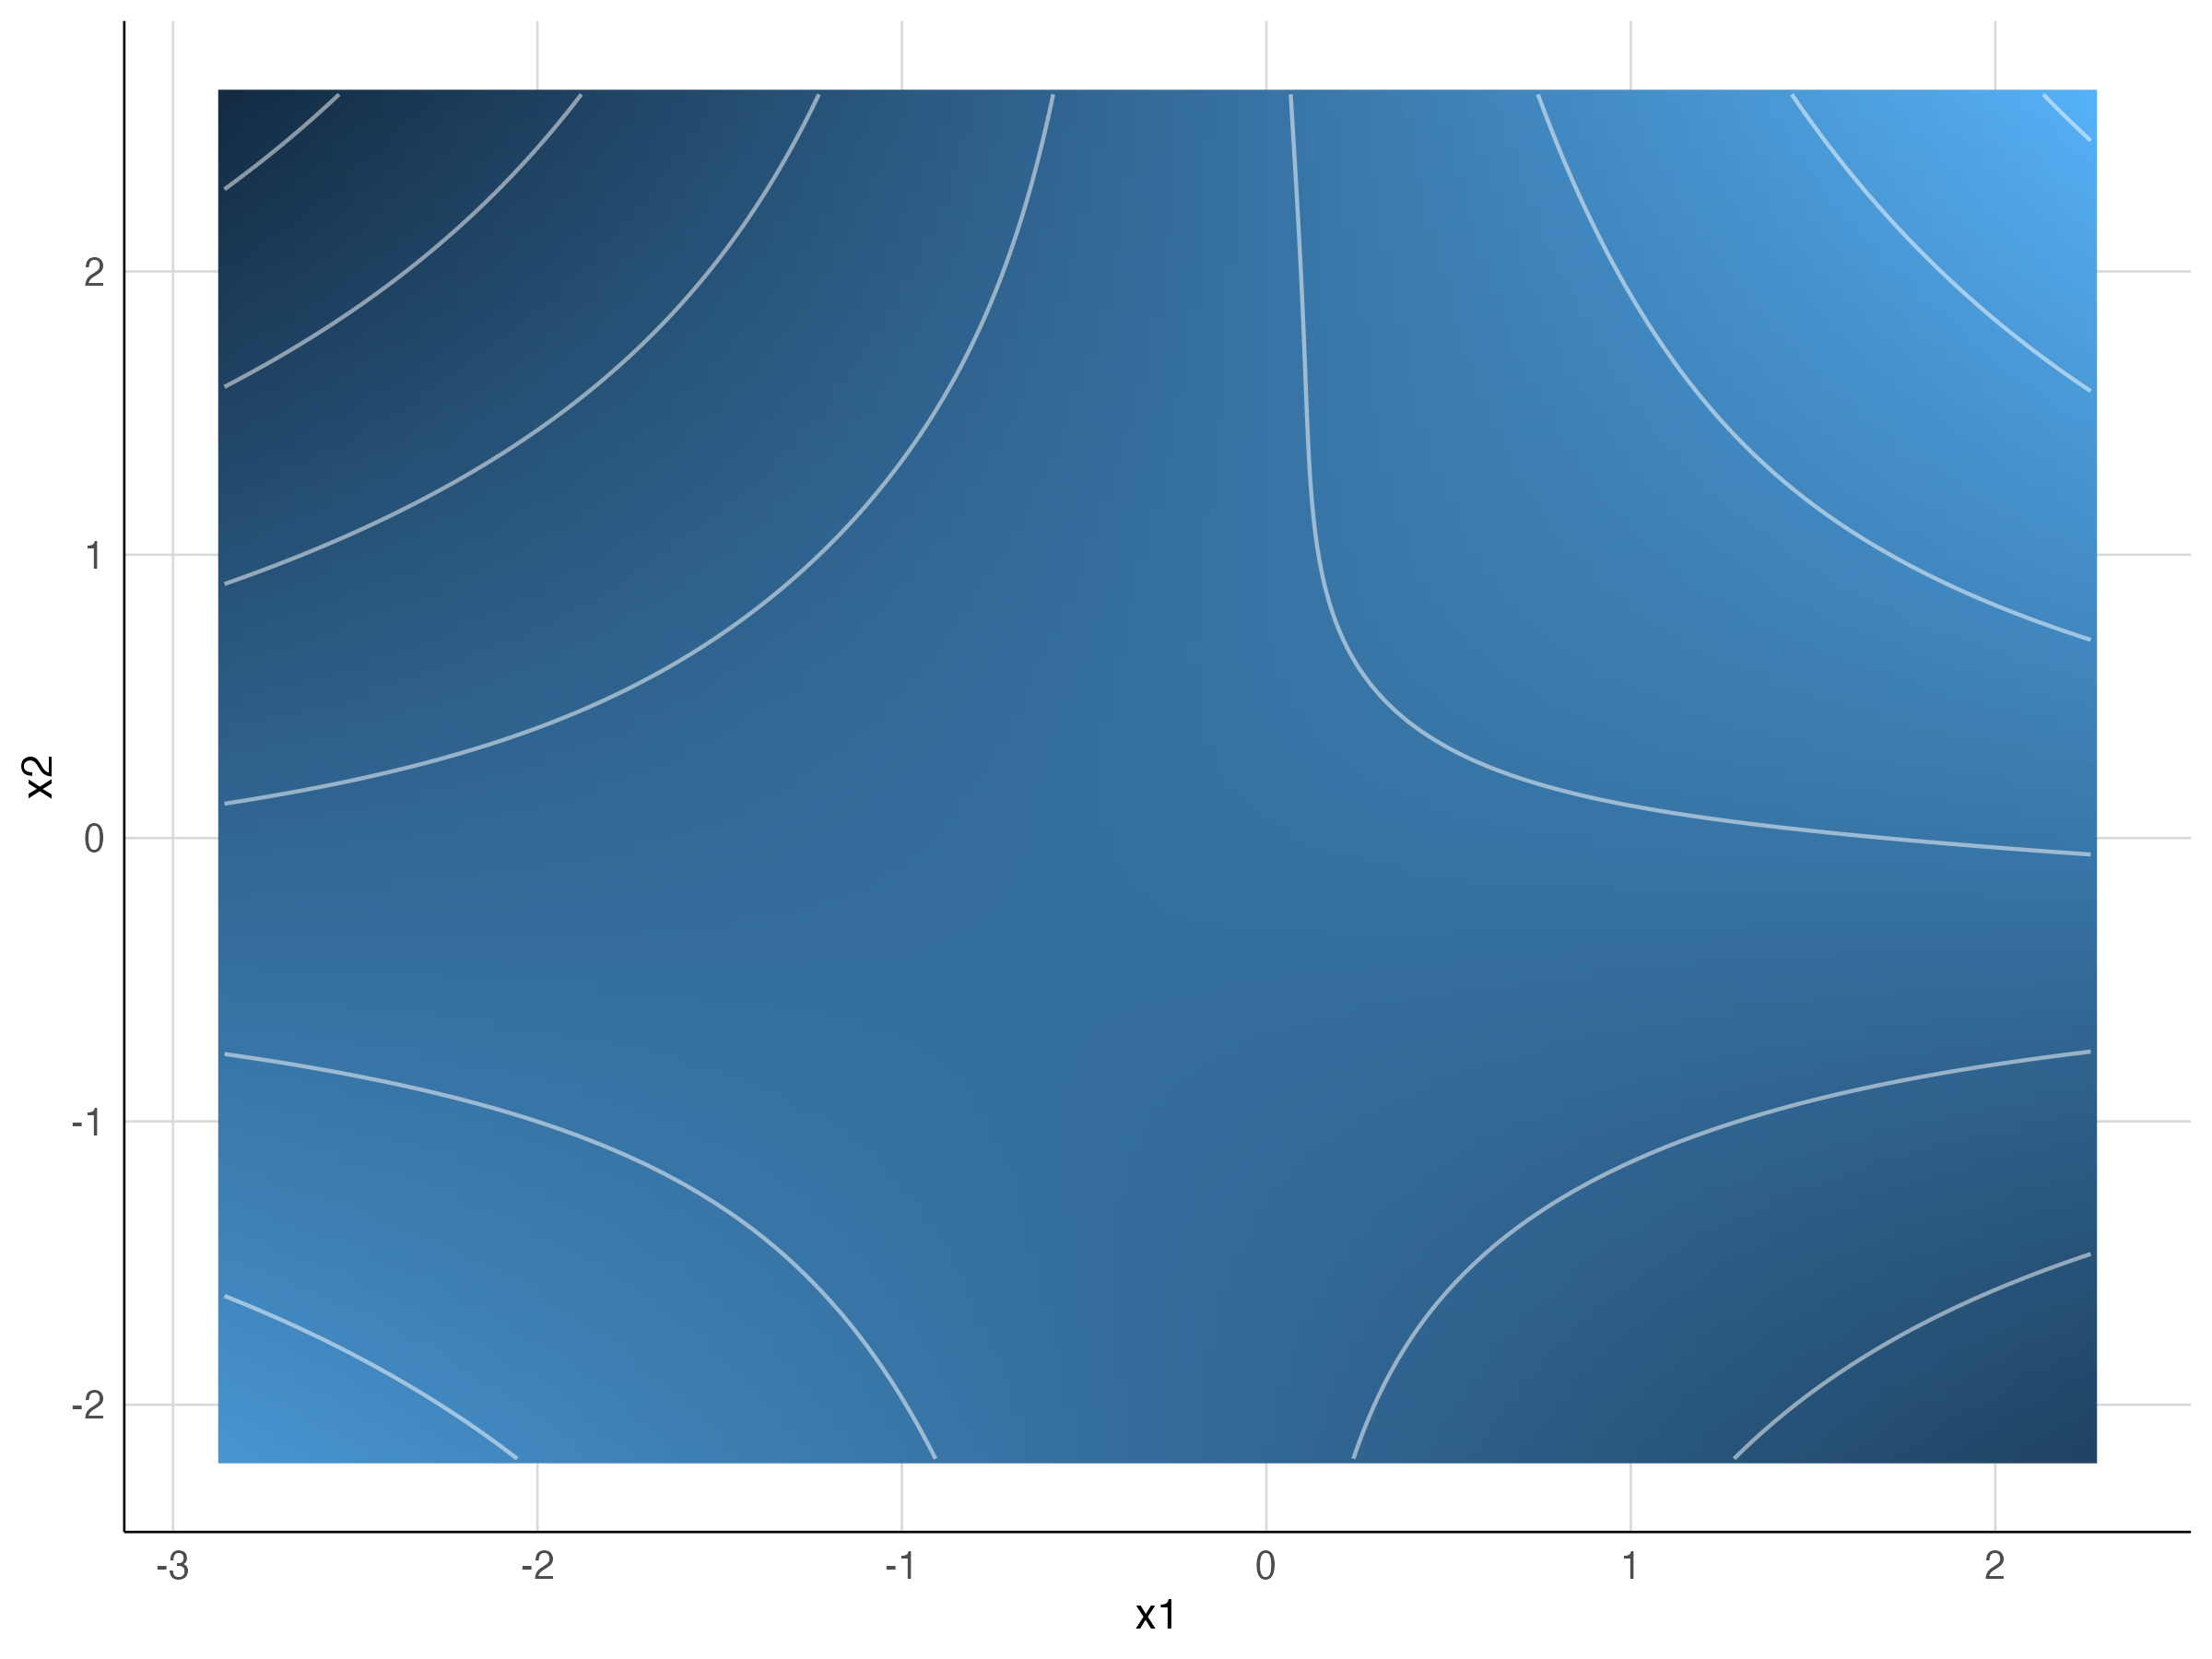
\includegraphics[width=\textwidth]{images/indep_150_interact.png}
%         \caption{Estimation of Contour plot of $g(x) = x_1 + 2 x_2 + x_1 x_2$ via Hooker method.}
%         \label{fig:indep_150_interact}
%     \end{minipage}
% \end{figure}

\subsubsection*{Standard MVN, linear function, interaction, dependent inputs}
% Zwei Plots für rho = 0.6 nebeneinander, jeweils halbe Breite
\begin{figure}[htpb]
    \centering
    \begin{minipage}[t]{0.49\textwidth}
        \centering
        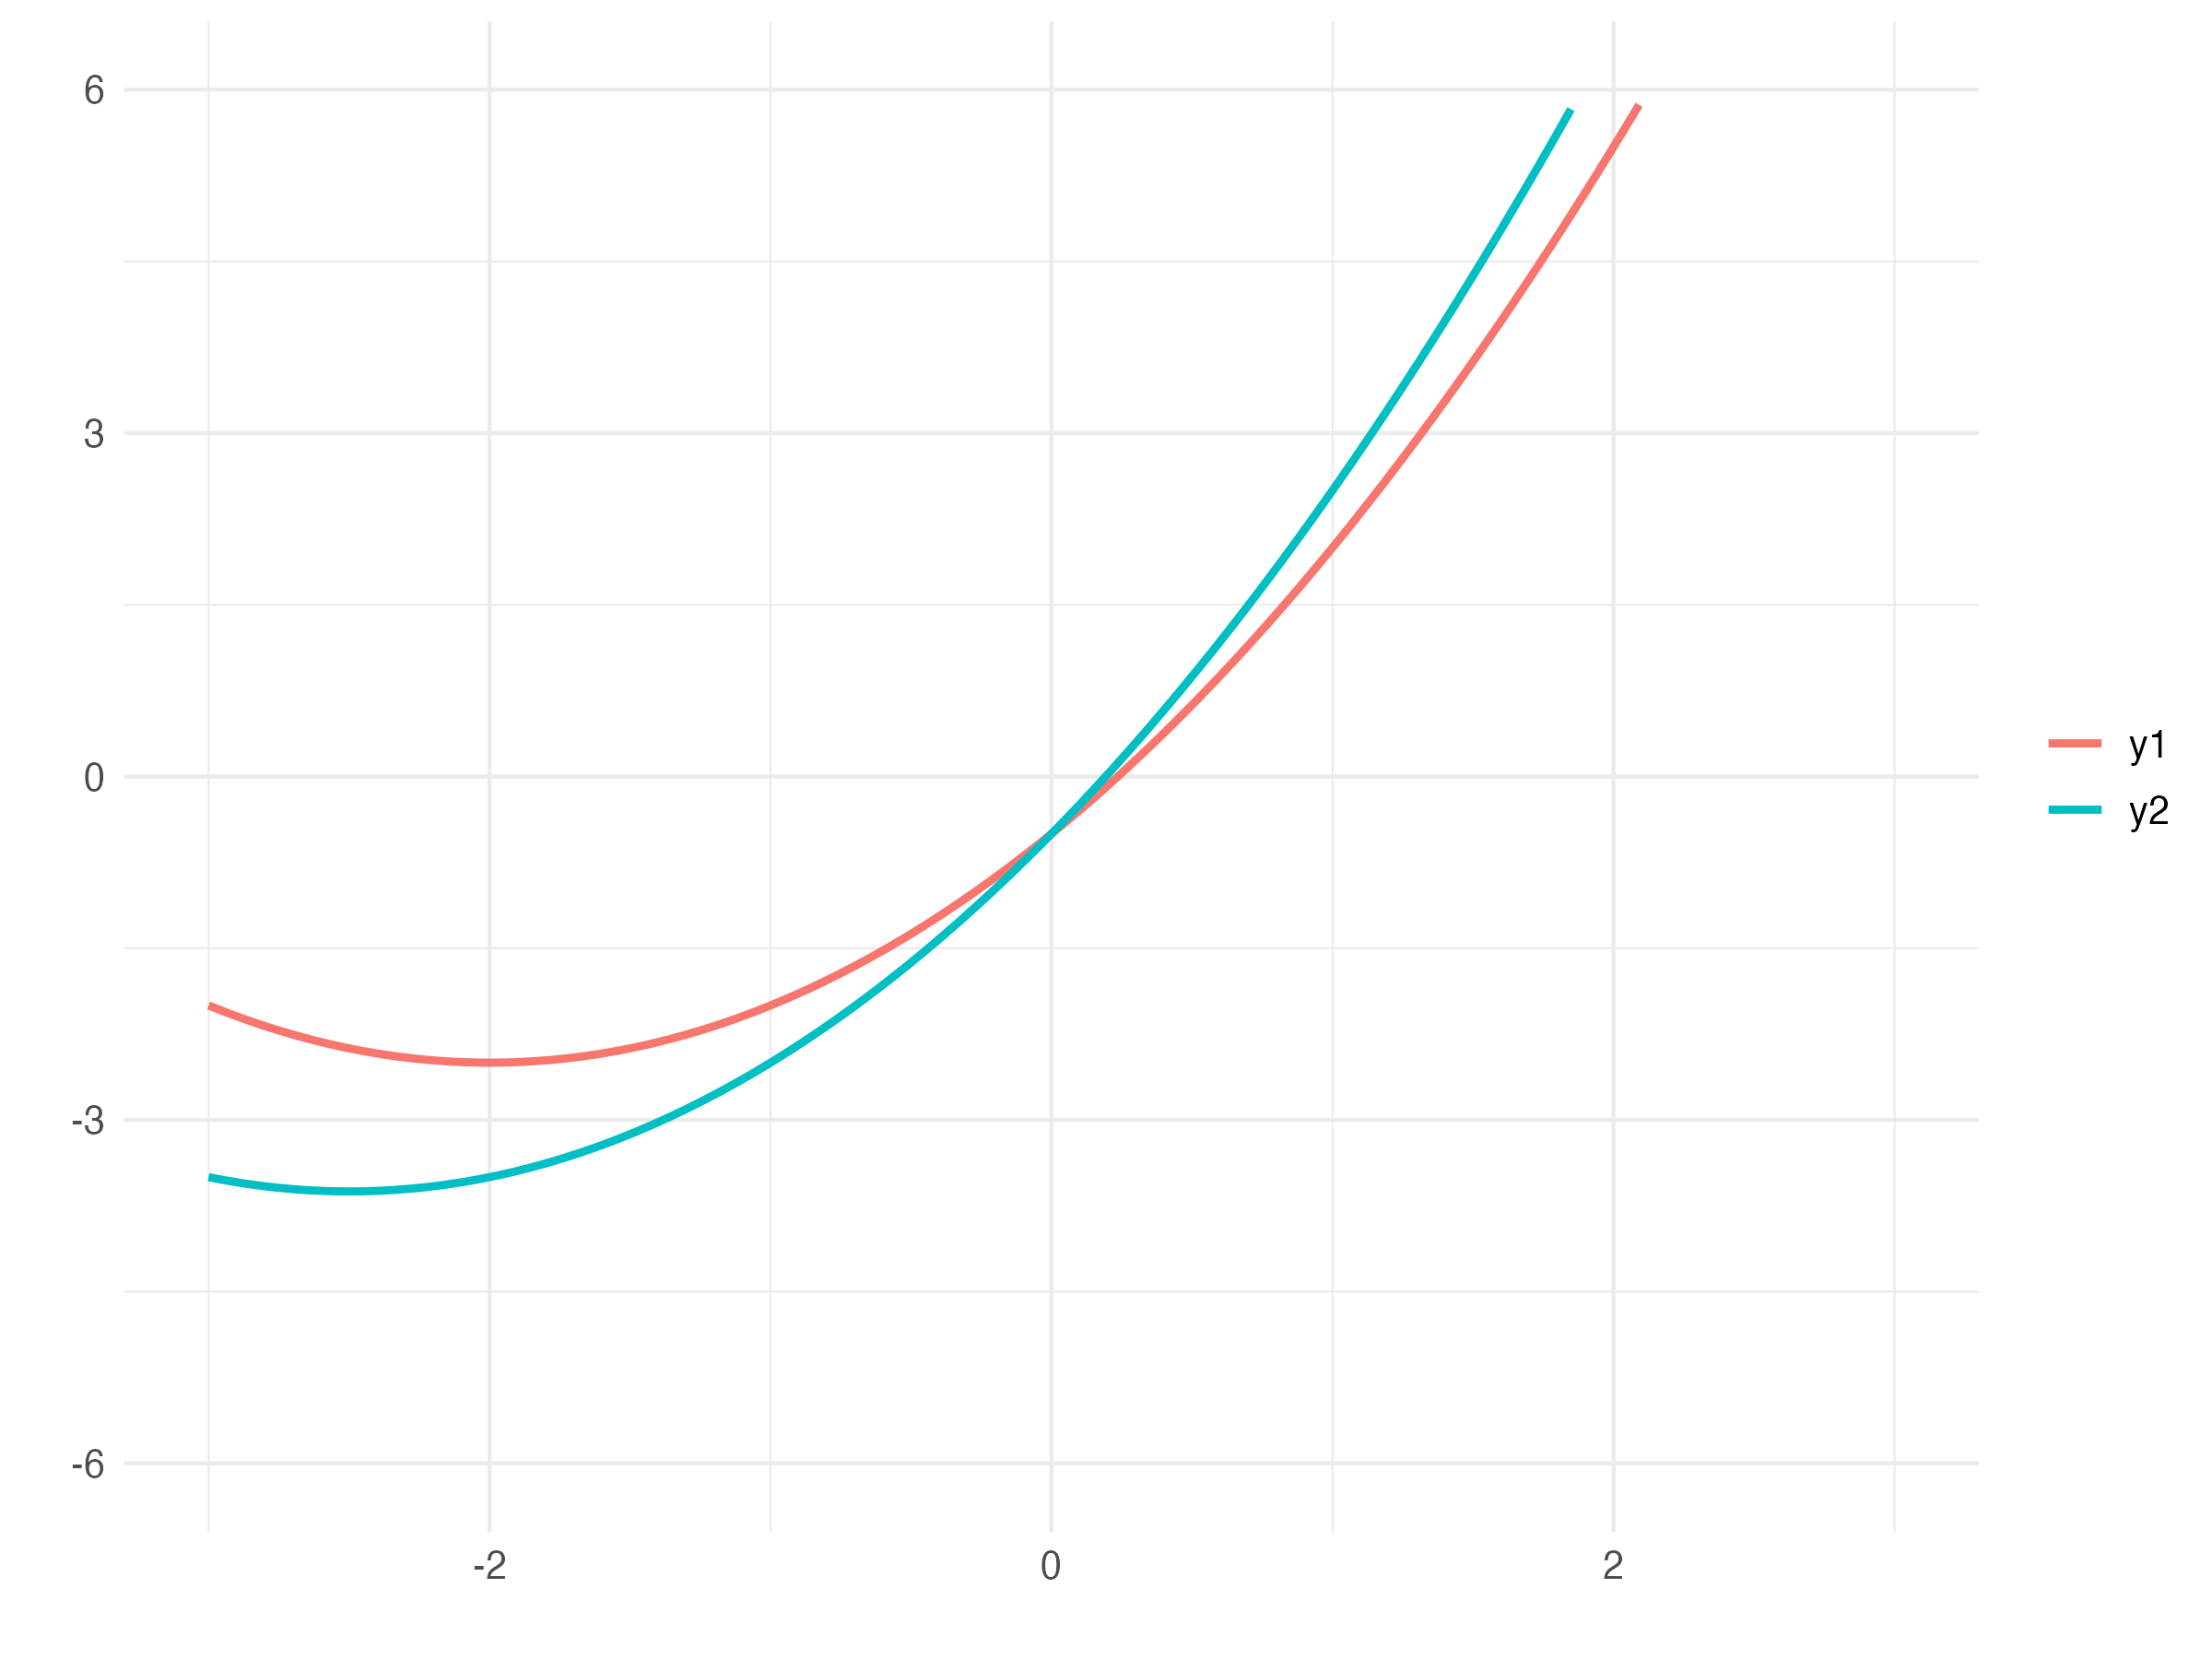
\includegraphics[width=\textwidth]{images/hoeffding_rho05.png}
        \caption{Hoeffding decomposition of $g(x) = x_1 + 2 x_2 + x_1 x_2$ with $\rho = 0.5$.}
        \label{fig:hoeffding_rho05}
    \end{minipage}%
    \hfill
    \begin{minipage}[t]{0.49\textwidth}
        \centering
        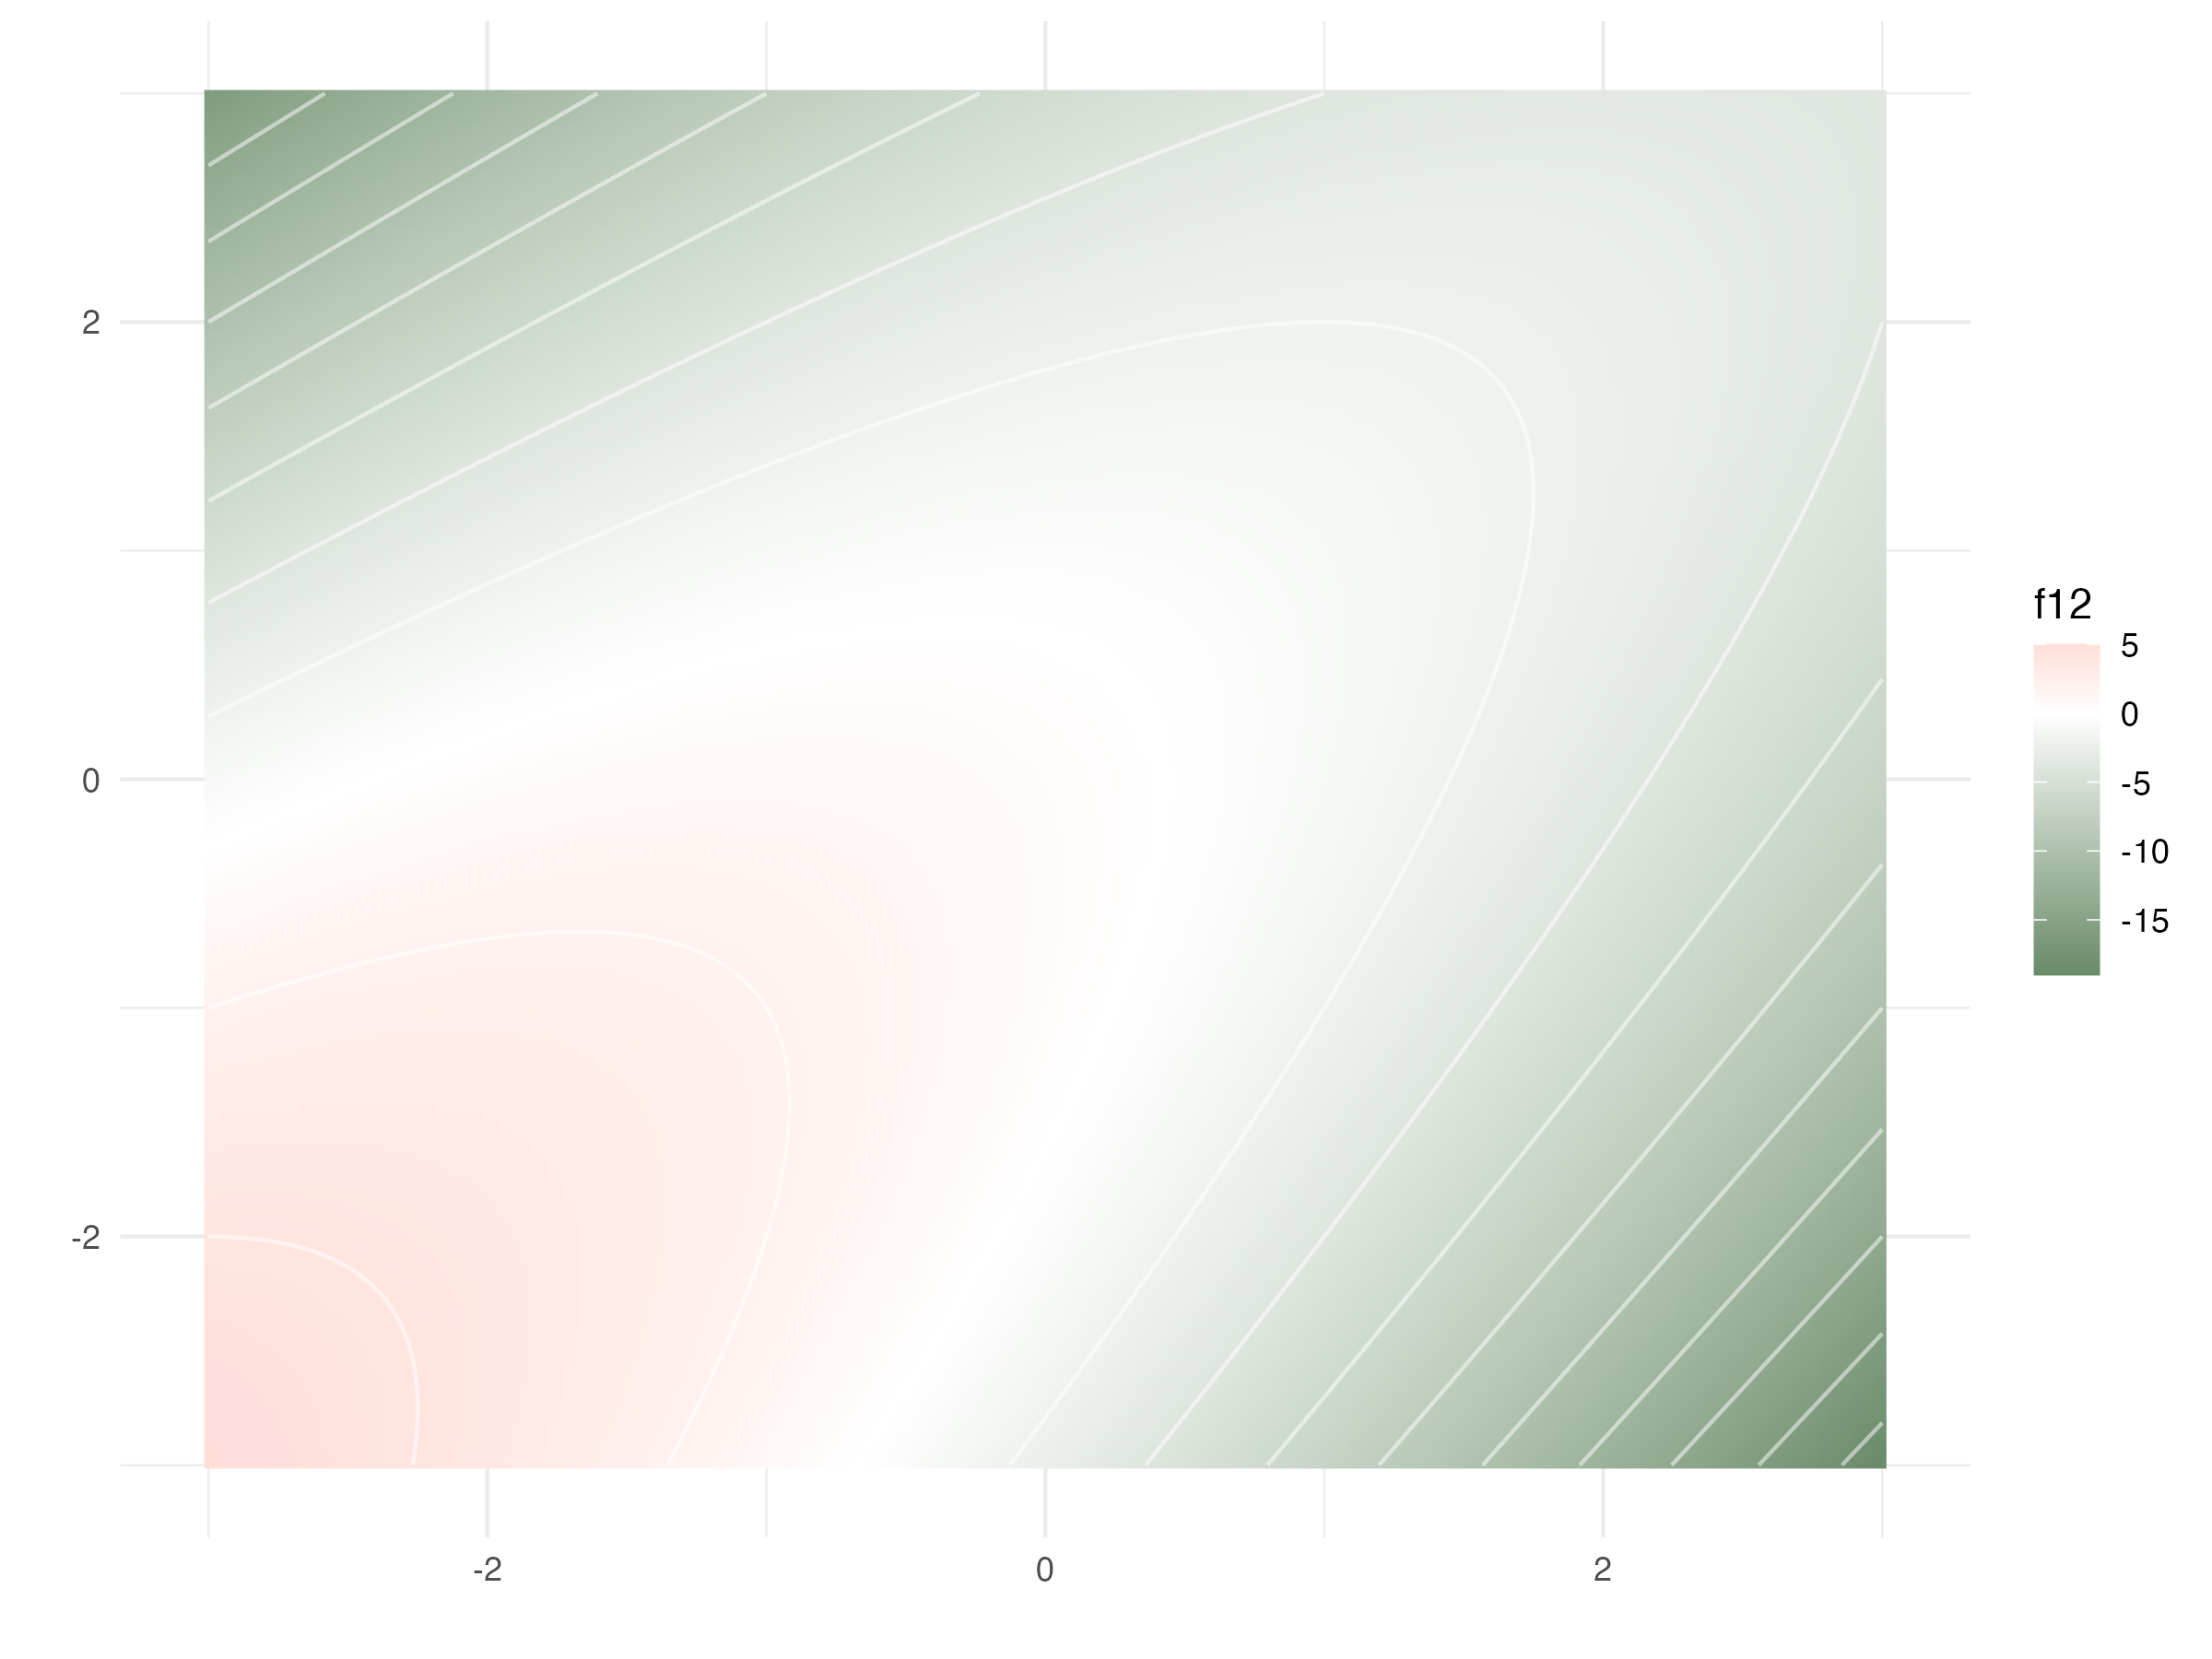
\includegraphics[width=\textwidth]{images/hoeffding_contour_rho05.png}
        \caption{Contour plot of $g(x) = x_1 + 2 x_2 + x_1 x_2$ with $\rho = 0.5$.}
        \label{fig:hoeffding_contour_rho05}
    \end{minipage}
\end{figure}

\subsubsection*{Estimated generalized fANOVA components}
\begin{figure}[htpb]
    % insert g1_1 and g1_2 as minipages
    \centering
    \begin{minipage}[t]{0.49\textwidth}
        \centering
        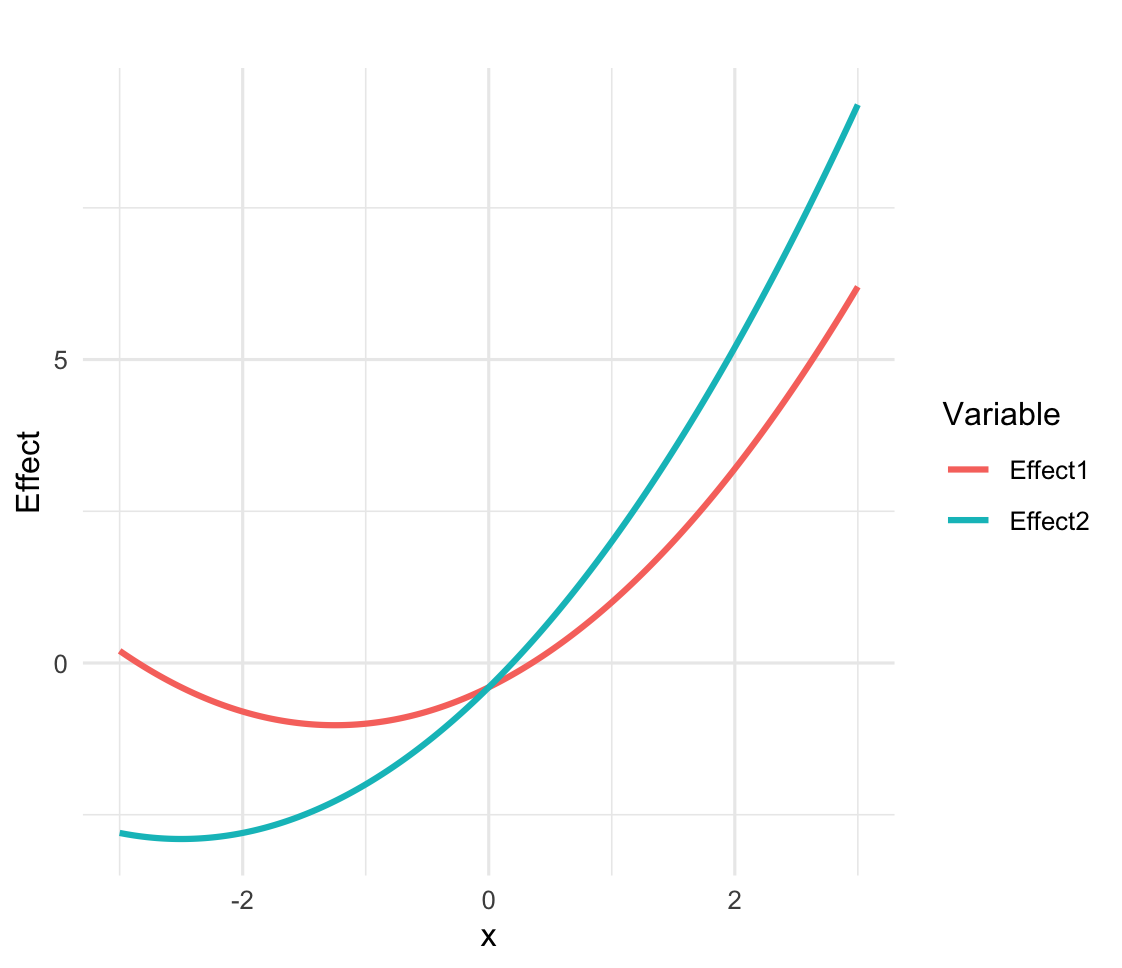
\includegraphics[width=\textwidth]{images/gpt_func_main.png}
        \caption{Generalized main effects for $g(x) = x_1 + 2 x_2 + x_1 x_2$ with dependent inputs, $\rho = 0.5$.}
        \label{fig:dep_150_main}
    \end{minipage}%
    \hfill
    \begin{minipage}[t]{0.49\textwidth}
        \centering
        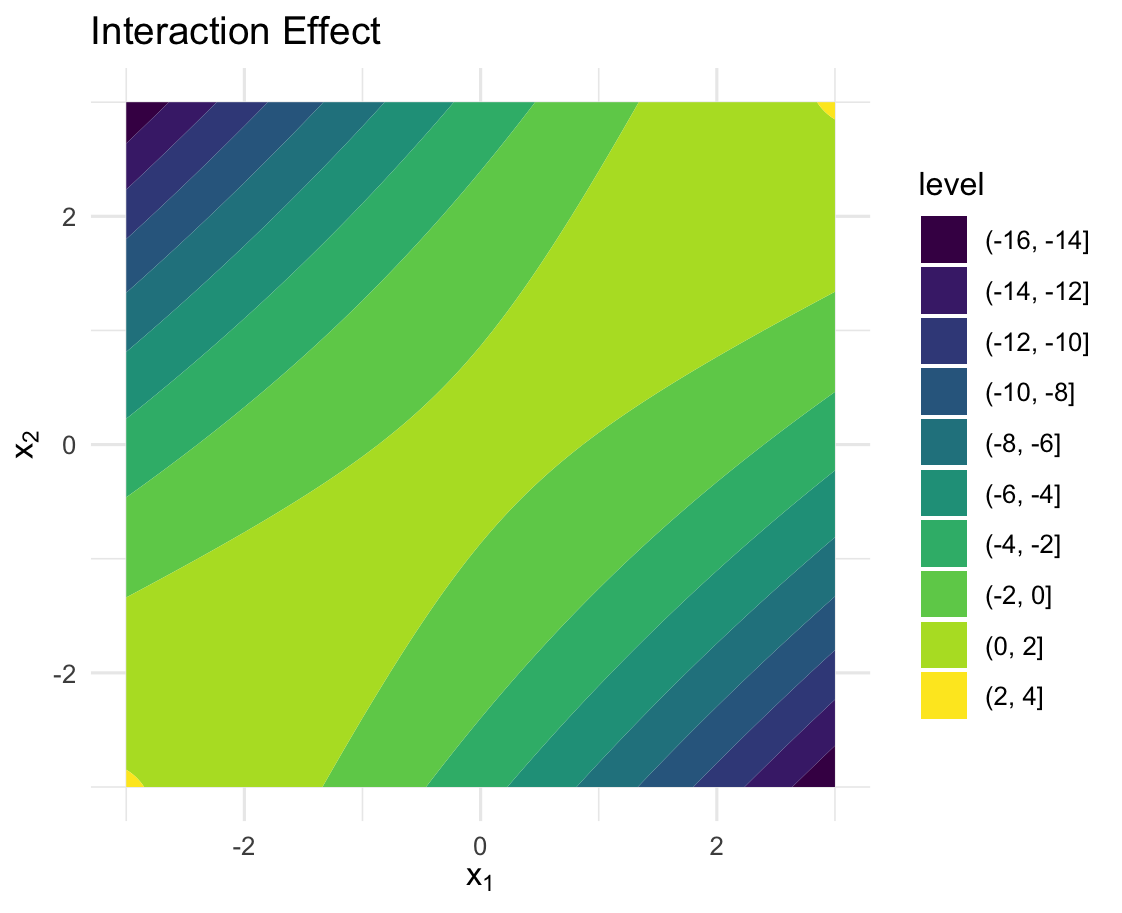
\includegraphics[width=\textwidth]{images/gpt_func_interaction.png}
        \caption{Contour plot of generalized interaction term for $g(x) = x_1 + 2 x_2 + x_1 x_2$ with dependent inputs, $\rho = 0.5$.}
        \label{fig:dep_150_interact}
    \end{minipage}
\end{figure}


\subsubsection*{Standard MVN, linear function, interaction, non-centred inputs}
Next, instead of a standard MVN distribution assumption for the inputs, we allow for non-centred inputs. This is to confirm that the fANOVA decomposition manages to yield zero mean components, even when inputs are not centred.
\(g = a + X_1 + 2X_2 + X_1 X_2\)
\[
\begin{pmatrix}
X_1 \\
X_2
\end{pmatrix}
\sim \mathcal{N}\left(
\begin{pmatrix} \mu_1 \\ \mu_2 \end{pmatrix},
\begin{pmatrix}
1 & 0 \\
0 & 1
\end{pmatrix}
\right).
\]
From the properties of the MVN, we know that marginal distributions are standard normal:
\[
X_i \sim \mathcal{N}(0, 1) \quad \text{for } i = 1, 2
\]

We also know that the conditional distributions are given by:
\[
X_1 \mid X_2 = x_2 \sim \mathcal{N}(\mu_1, 1), \quad
X_2 \mid X_1 = x_1 \sim \mathcal{N}(\mu_2, 1)
\]

We can now compute the classical fANOVA components as follows:
\begin{align*}
    y_{\emptyset} &= \mathbb{E}[g(X)] = a + \mu_1 + 2\mu_2 + \mu_1 \mu_2, \\
    y_1 &= \mathbb{E}[g(X) \mid X_2 = x_2] - y_{\emptyset}= a + 2\mu_2 + x_1 + x_1 \mu_2 - y_{\emptyset} \\
    &= x_1 ( 1 + \mu_2) - \mu_1 \mu_2 - \mu_1, \\
    y_2 &= \mathbb{E}[g(X) \mid X_1 = x_1] - y_{\emptyset} = a + \mu_1 + 2x_2 + x_2 \mu_1 - y_{\emptyset} \\
    &= x_2 (2 + \mu_1) - \mu_1 \mu_2 - 2 \mu_2, \\
    y_{12} &= g(x_1, x_2) - y_{\emptyset} = x_1x_2 - \mu_2 x_1 - \mu_1 x_2 + \mu_1 \mu_2.      
\end{align*}
We recognize that each fANOVA components is shifted by constants (that are formed from the conditional and unconditional expected values of the input variables). 

It is easy to verify that non-constant terms have mean zero:
\begin{align*}
    \mathbb{E}[y_1] &= \mathbb{E}[X_1 (1 + \mu_2) - \mu_1 \mu_2 - \mu_1] = (1 + \mu_2) \mathbb{E}[X_1] - \mu_1 \mu_2 - \mu_1 = 0, \\
    \mathbb{E}[y_2] &= \mathbb{E}[X_2 (2 + \mu_1) - \mu_1 \mu_2 - 2\mu_2] = (2 + \mu_1) \mathbb{E}[X_2] - \mu_1 \mu_2 - 2\mu_2 = 0, \\
    \mathbb{E}[y_{12}] &= \mathbb{E}[X_1X_2] - \mu_2 \mathbb{E}[X_1] - \mu_1 \mathbb{E}[X_2] + \mu_1 \mu_2 = 0.
\end{align*}
Varying the mean of MVN inputs will result in shifted fANOVA components. Varying the variance of intput variables will not change the fANOVA decomposition and is therefore not investigated further.
% Input: Poisson/ Exponential/ Beta/ etc. not centred, independent

\paragraph{Non-additive functions}
These functions demonstrate that fANOVA does not assume additive structure and can identify purely interactive effects. If variables only appear in interaction terms, their main effects vanish:
\[
f_2(x) = x_1 \cdot x_2 \cdot x_3 \cdot x_4
\]


\subsubsection*{Uniform, quadratic, no interaction}
Let us also try out another function $g(x_1, x_2) = a + x_1 + x_2^2$; to see how fANOVA deals with quadratic main effects. 
We will also change the distribution of the inputs. Lets us consider two independent random variables with uniform distribution over the interval \([-1, 1]\), meaning they are already centred. We calculate:
\begin{align*}
y_\emptyset &= \mathbb{E}[g(X_1, X_2)] = a + \mathbb{E}[X_1] + \mathbb{E}[X_2^2] = a + 0 + \tfrac{1}{3} = a + \tfrac{1}{3} \\
y_1(x_1) &= \mathbb{E}[g(x_1, X_2)] - y_\emptyset = a + x_1 + \tfrac{1}{3} - \left(a + \tfrac{1}{3}\right) = x_1 \\
y_2(x_2) &= \mathbb{E}[g(X_1, x_2)] - y_\emptyset = a + 0 + x_2^2 - \left(a + \tfrac{1}{3}\right) = x_2^2 - \tfrac{1}{3} \\
y_{1,2}(x_1, x_2) &= g(x_1, x_2) - y_\emptyset - y_1(x_1) - y_2(x_2) = a + x_1 + x_2^2 - \left(a + \tfrac{1}{3} + x_1 + x_2^2 - \tfrac{1}{3}\right) = 0
\end{align*}
